\chapter{Web-page User Interface}\label{ch:5}

To keep the development of the front-end as simple as possible, a single-page structure for the web-page was used.
Upon visiting the page, the user is presented with a multi-parameter form for querying repositories.
Once the parameters have been set, searching would reveal a list of repositories matching the specified criteria.
Results are presented in batches of 20 matching repositories at a time, with the options to navigate to each of the result pages, as well as download the full result list in file format.
The following sections will be dedicated to explaining the website structure and mechanics.

\section{Search Form}

Each repository search begins with specifying the sampling criteria.
To better communicate searchable repository characteristics to the user, it was necessary to design an organised and comprehensive search form.
The final adopted design can be seen in Figure~\ref{fig:3}.
The search form filters are grouped into 5 major sections:
\begin{itemize}
    \item \textit{General filters}
    \\These include text-based filters for filtering repositories by name, license, label used and main language. The name filter can also be toggled to either match repositories containing a keyword (non case-sensitive), or to match by fully qualified repository name (\code{user_name/repo_name}, which is case-sensitive). The remaining inputs use a typeahead to aid the user in selecting the desired license/label/language to filter by.
    \item \textit{History and Activity filters}
    \\These include numerical range filters for selecting repositories by number of commits, contributors, issues (total), pull requests (total), branches and releases, each query parameter having a minimum and maximum range restriction value. Keep in mind that selection ranges are inclusive, meaning that searching any parameter by a minimum of $n$ and a maximum of $m$ yields all results belonging to the interval $[n,m]$. The chevron arrows next to the inputs can be used to increment or decrement the current value of a field.
    \item \textit{Date-based filters}
    \\These include date range filters that allow selecting repositories by date of creation and last commit. The input format for date searches is \textit{YYYY-MM-DD}, with the time of the selected dates being automatically set to midnight (For example, querying for repositories created after \textit{2011-03-08}, will yield all the mined repositories created after \textit{2011-03-08 00:00:00}). Like the other numerical filters, date filters are also inclusive. Date inputs also employ calendar-style date pickers to aid in date selection.
    \item \textit{Popularity filters}
    \\These include numerical range filters for selecting repositories by number of stars, watchers and forks. They function in the exact same way as the \textit{History and Activity filters} do.
    \item \textit{Additional filters}
    \\These include boolean filters that allow selecting forks or source projects exclusively, as well as minimising selections to repositories containing open issues, open pull requests, a wiki, or a license.
\end{itemize}

\begin{figure}[ht!]
    \centering
    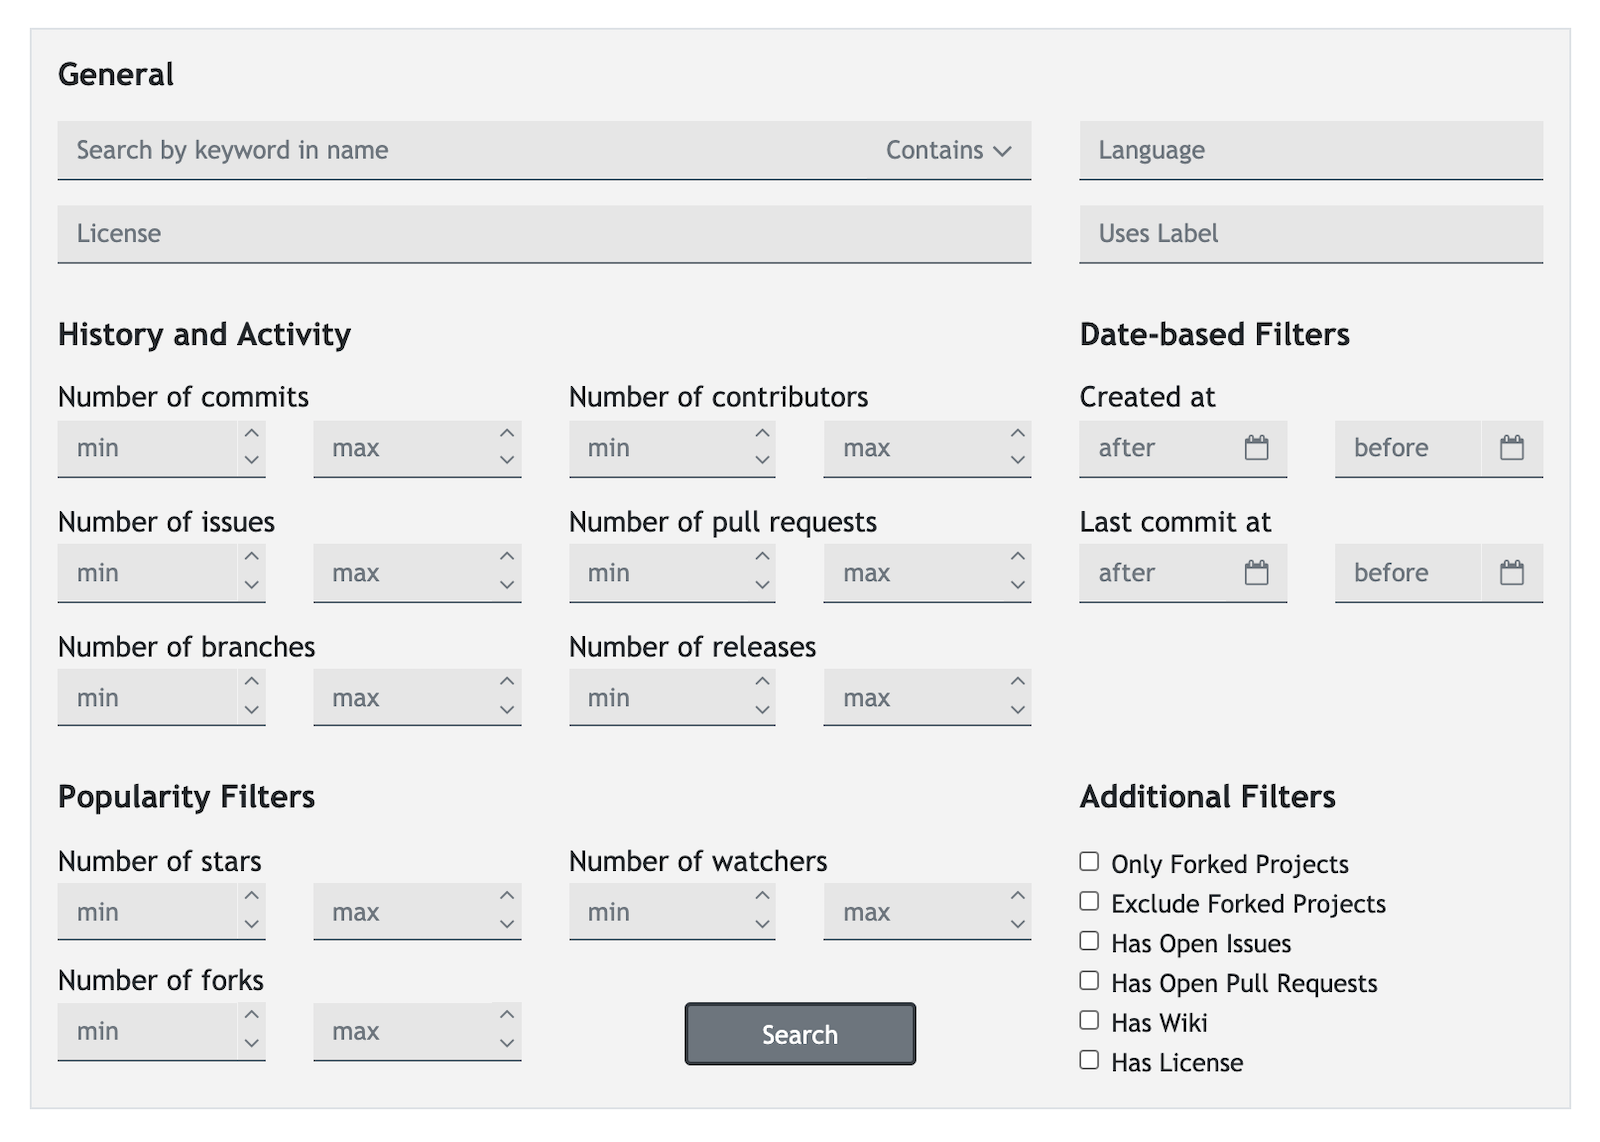
\includegraphics[width=1\linewidth]{form}
    \caption[Search form]{The search form.}
    \label{fig:3}
\end{figure}

To prevent the user form providing illegal inputs, the from uses a basic RegEx input verification.
Inputs containing non-supported characters will immediately change their background colour to red.
If the user still attempts to submit queries with incorrectly formatted parameters, then the form explicitly points to the fields who's inputs need to be changed, via a popup.
It is also worth mentioning that all the form parameters are optional, meaning that searching right off the bat will yield a result set of all repositories currently stored in the database.

\begin{figure}[ht!]
    \centering
    \begin{minipage}[b][][b]{0.60\textwidth}
        \centering
        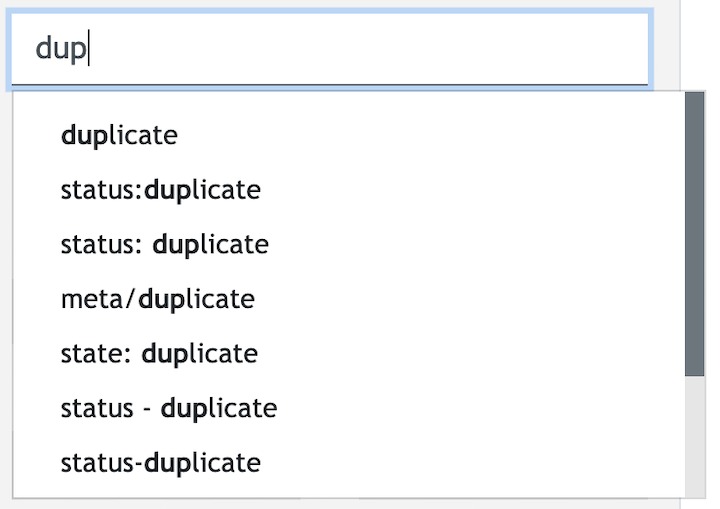
\includegraphics[width=1\linewidth]{typeahead}
        \caption*{a)}
    \end{minipage}\hfill
    \begin{minipage}[b][][b]{0.40\textwidth}
        \centering
        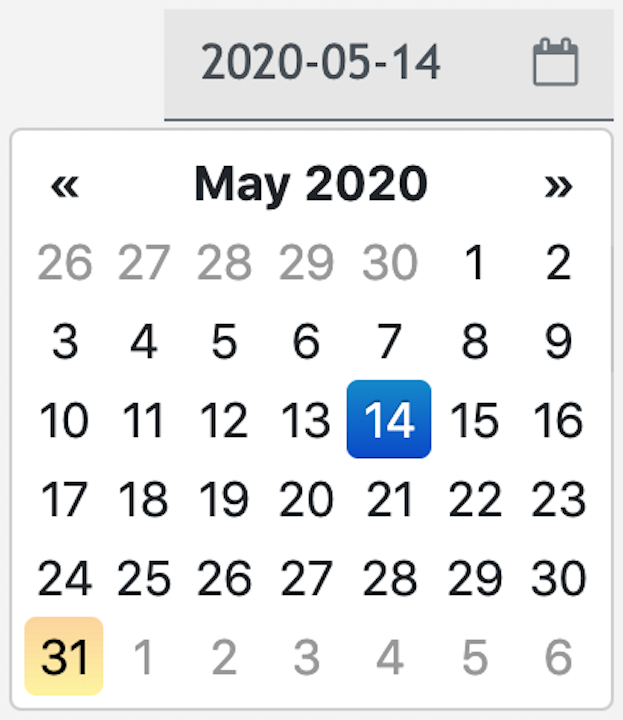
\includegraphics[width=1\linewidth]{datepicker}
        \caption*{b)}
    \end{minipage}
    \label{fig:4}
    \caption[Form input typeahead and date picker]{a) The typeahead used for suggesting labels. Letters highlighted in the input correspond to the input match. b) The date picker used in the date-based filters. The blue selection marks the currently selected date, while the yellow selection marks the current date.}
\end{figure}

\newpage
\section{Result List}

Following the query submission, the search form is hidden to reveal a list of matching results to the user.
To keep the querying performance constant, the full result set is broken up into pages consisting of 20 items per page, with the total number of results and the current page shown at the top of the result list (an example is shown in Figure~\ref{fig:6}).
Naturally, if the user is satisfied with the presented results, the links to download the full list of results in either of the three supported file formats are included on the top of each result page.

Given that the rudimentary sampling process requires the researcher to review a subset of the presented information, it was necessary to include options for page traversal.
Therefore, navigation links were included at the bottom of the result list (seen in Figure~\ref{fig:7}), and include three traversal categories:
\begin{itemize}
    \item Moving by one page (Which is either to the next or previous result page);
    \item Moving to the start or end of the results (Which is either the first or last result page); and
    \item Moving to any desired page, specified by the user through a single-input form.
\end{itemize}
Links are also configured not to lead the user to an invalid page. For example: the links to the first or previous page will not be displayed if the user is on the first page. This also applies to next and last page links. The page jumping input only accepts numerical arguments ranging from 0, to the number of the last page. Like the search form inputs, it also uses color changes and popups to communicate incorrect data formatting to the user. Furthermore, all navigation and download links are disabled for searches yielding no results (as seen in Figure~\ref{fig:5}).

\newpage
\begin{figure}[ht!]
    \centering
    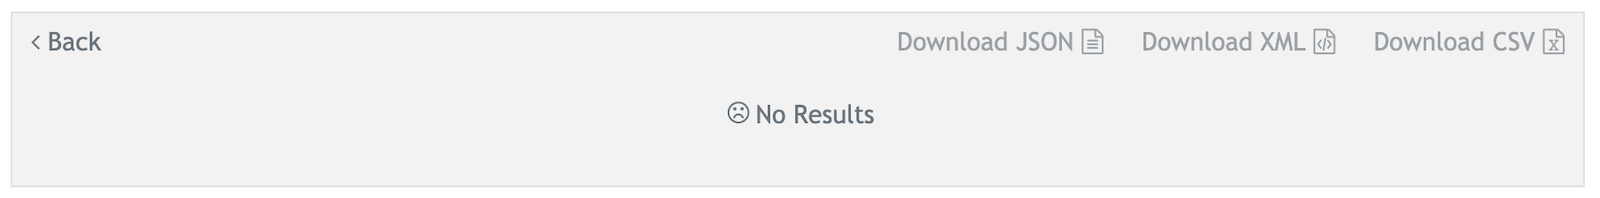
\includegraphics[width=1\linewidth]{no_results}
    \caption[Empty result list]{A search yielding no results.}
    \label{fig:5}
\end{figure}

\begin{figure}[ht!]
    \centering
    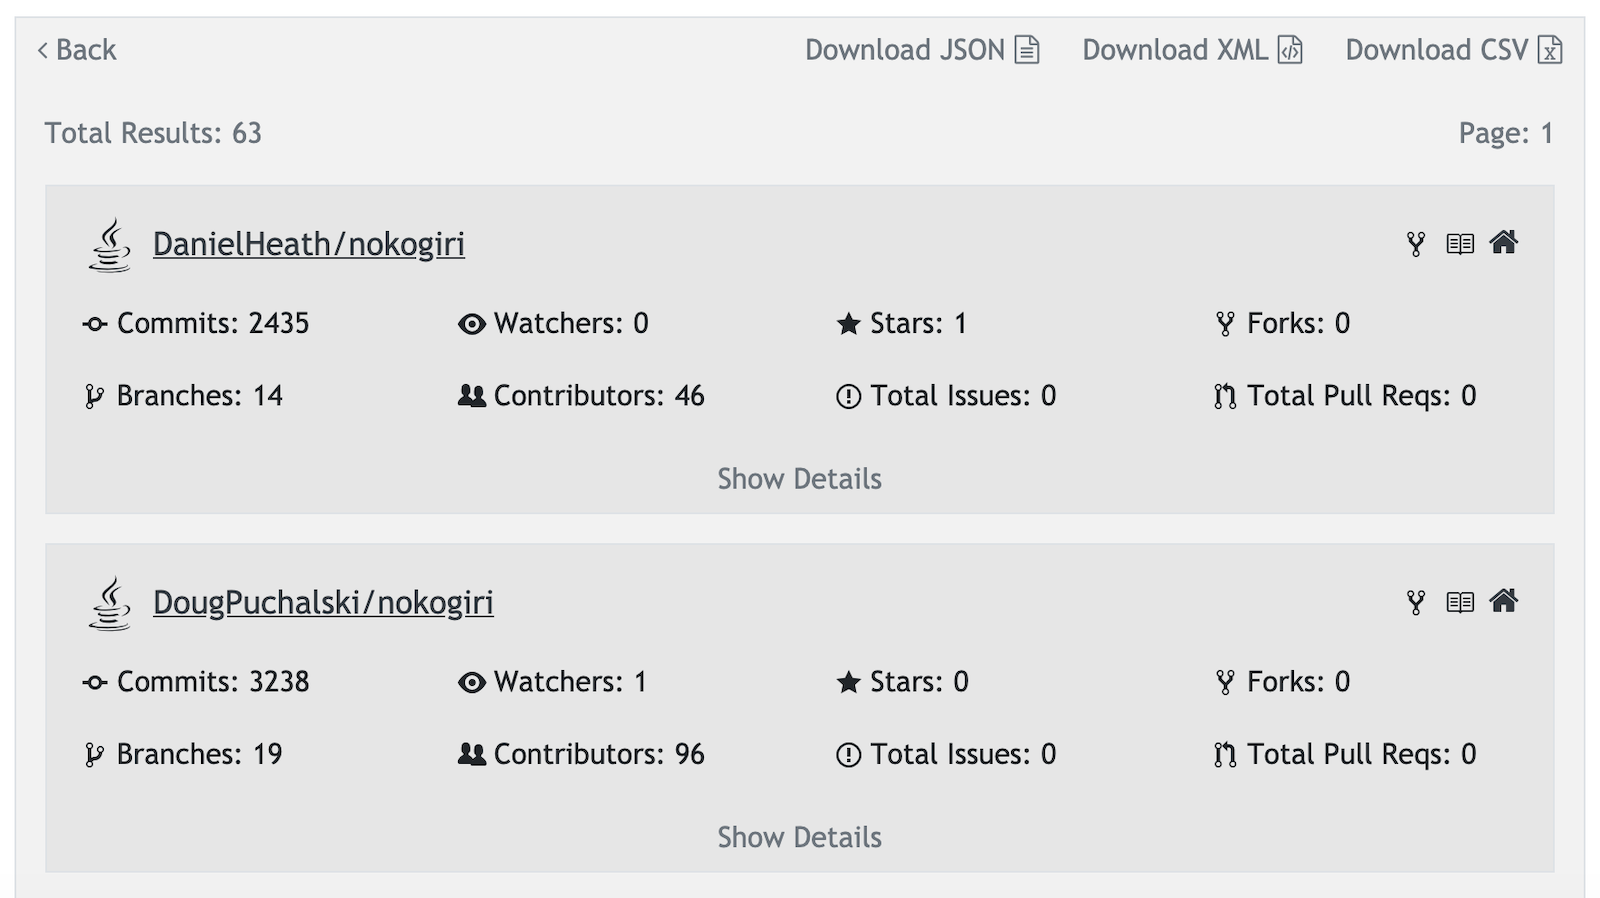
\includegraphics[width=1\linewidth]{results}
    \caption[Search result list]{The top of the search result list for repositories containing the keyword ``nokogiri''.}
    \label{fig:6}
\end{figure}

\begin{figure}[ht!]
    \centering
    
\includegraphics[width=1\linewidth]{navigation}
    \caption[Search page navigation options]{The page navigation options displayed on the bottom of the result list.}
    \label{fig:7}
\end{figure}

\newpage
\section{Result Item}

The challenge with designing the layout of a result list item, is finding the most optimal layout configuration for all data retrieved for a repository.
Defining the priority of information presented helps with tackling this issue.
For example stats such as the repository name, main language, commit, star and contributor count have a higher significance compared to default branch name or date of last update.

Furthermore, presenting the user with information without the use of plain text also helps minimise the amount of required space.
This where icons come in to play, as they can be used to visually present concepts to the user without the need for verbosity.
Using GitHub's default icon set, commonly referred to as Octicons, made sense as those already familiar with GitHub will be able to easily recognise the icons, and easily infer the meaning of the data they are associated with.
Even if a user was unfamiliar with the icon itself, hovering over it would reveal its meaning.
Icons also help with the abbreviation of presented data.
Rather than including a separate row for displaying the main language of a repository, the interface instead uses a language icon next to the repository name.

Finally, it is important to increase the overall readability of the result set.
Rather than bombarding the user with all repository information, only the most important information is presented upfront, with the remainder supplied to the user on demand.
Toggling the hidden information is implemented through a collapsible bootstrap component, which at the push of a button can either show or hide information.

Figures~\ref{fig:9} and~\ref{fig:10} show the final adopted design for result items.
Information such as the repository main language and name are displayed displayed on top, followed by icons showing project status (shown in Figure~\ref{fig:8}), such as if it is archived, whether it is a fork, whether it has a wiki and a homepage.
Keep in mind that the aforementioned status icons are optional, and may not be displayed if the repository does not have these statuses.
The repository name and homepage icon also act as links that direct the user to the GitHub project page and external homepage in a new browser window.

\begin{wrapfigure}{r}{5cm}
    \centering
    
\includegraphics[width=5cm]{status_icons}
    \caption[Status icons]{Status icons.}
    \label{fig:8}
\end{wrapfigure}

The next four rows are dedicated to statistical information, each row containing four columns dedicated to a single data point.
A data point consists of a distinct icon, followed by a label for the data, and finally the values themselves.
Next up are the license (displayed only if a project is licensed), last commit SHA and default branch rows, similarly formatted to previous rows.
Finally project languages and labels are separated in their own sections.
Said sections only appear if a project has more than one used language or one or more labels respectively.

\begin{figure}[ht!]
    \centering
    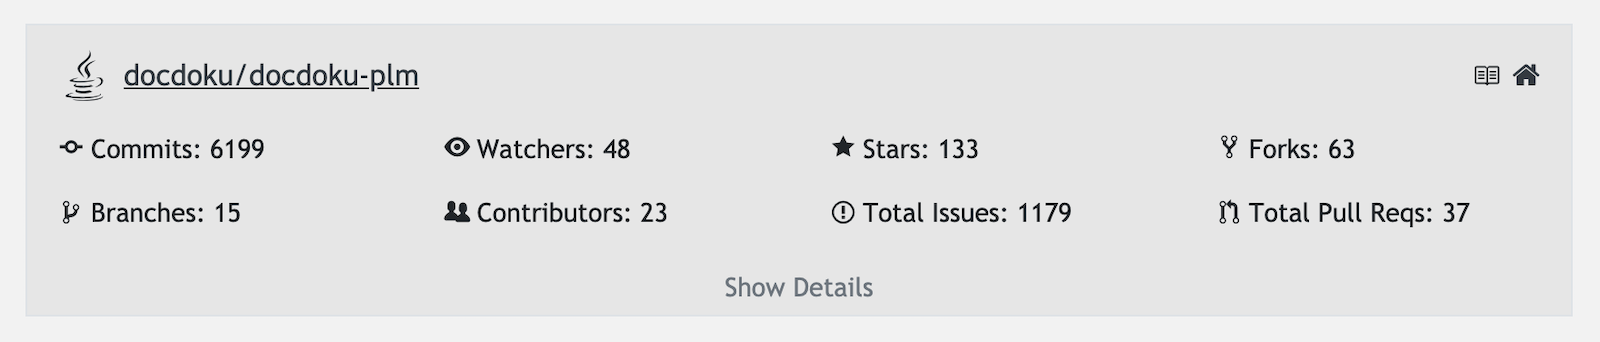
\includegraphics[width=1\linewidth]{result_partial}
    \caption[Result item partial]{A result item showing only basic information.}
    \label{fig:9}
\end{figure}

\begin{figure}[ht!]
    \centering
    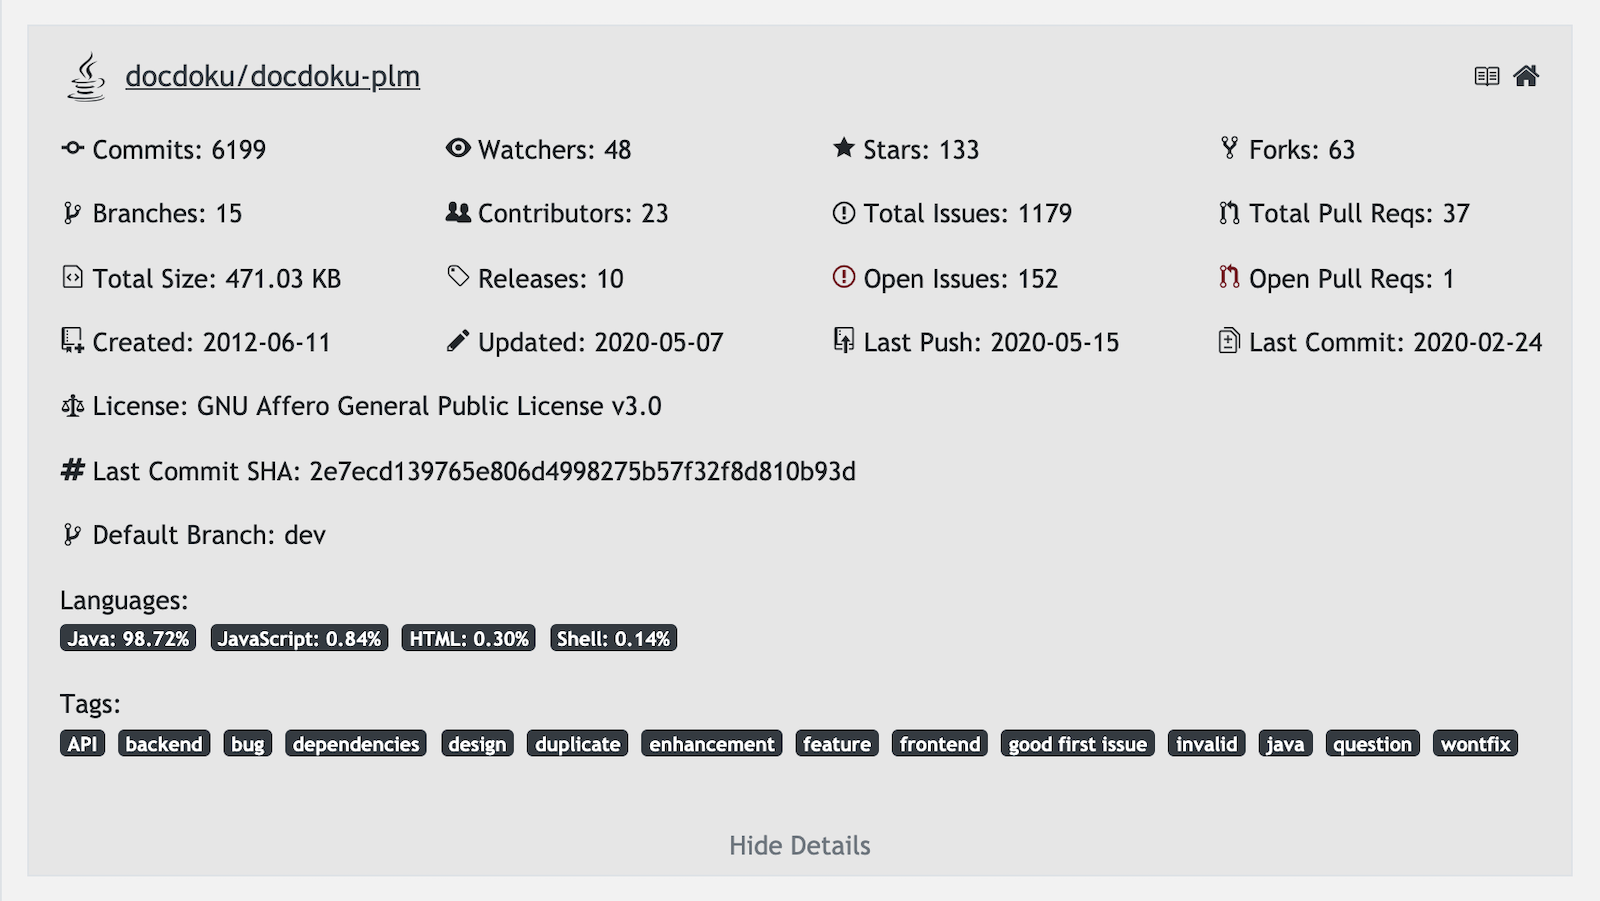
\includegraphics[width=1\linewidth]{result_full}
    \caption[Result item full]{All information contained within a result item.}
    \label{fig:10}
\end{figure}